% !TeX root = ../../../Main.tex

\chapter{Appendix}
\section{Glider Parameters}
\label{appendix_A}

\begin{table}[h]
	\begin{center}
		\begin{tabular}{r|l}
			mass m& $3.366 kg$\\
			wing area S & $0.568 m^2$ \\
			aspect ratio $\Lambda$ & $10.2$ \\
			oswald efficiency factor e& $0.9$ \\
			$c_{D0}$ & 0.015 \\
		\end{tabular}
		\caption{glider data}
		\label{tab:glider_data}
	\end{center}
\end{table}

\newpage
\section{Computer Configuration and Implementation}
\label{appendix_B}
\subsection{Computer Configuration}
Table \ref{tab:pc_specs} contains the technical data of the computer used for the calculations.

\begin{table}[h]
	\begin{center}
		\begin{tabular}{r|l}
			CPU & Intel i7-7700HQ @ 2.80 GHz (4 physical cores, 8 threads) \\
			RAM\nomenclature[A]{RAM}{random access memory} & 16 GB DDR3 RAM @ 3200 MHz \\
			GPU & Nvidia Geforce GTX 1050 Ti (4 GB VRAM, 768 CUDA cores) \\
			OS & Ubuntu 16.04 LTS
		\end{tabular}
	\caption{computer specifications}
	\label{tab:pc_specs}
	\end{center}
\end{table}

All algorithms were implemented in Python (Version 3.5), utilizing the rllab framework \cite{rllab2018}. The policy ANN used in the simulations was handled by the GPU\nomenclature[A]{GPU}{graphics processing unit} using CUDNN, Theano and Lasagne. All other code including the tables representing the greedy actions and state values was executed with eight parallel processes on the CPU\nomenclature[A]{CPU}{central processing unit}. \smallbreak

The rllab framework already contains a step-method that lets the agent make a step through the state space. The original step method takes the current state $s_t$ of the agent, which is stored as a class attribute, and an action $a_t$, which is passed in the function call. It returns the next state $s_{t+1}$, the reward $r_{t+1}$ and a flag telling the agent whether he has reached a terminal state. This step-method has been modified so it also takes the current state $s_t$ as an argument. This way, a one step lookahead can be performed from any state regardless of the state that is currently stored in the class attribute.

\subsection{Computational Subtleties of PI and VI}

As mentioned in chapter~\ref{chapter7}, a value iteration takes less time than a policy iteration. This is due to a few subtle differences between VI and PI. In every Policy Iteration step, the following actions are performed for each state:

\begin{itemize}
	\item Update the state value by performing a one step lookahead with the current greedy action (cf. Eq.~\ref{eq:bellman_exp_update_bootstrapped}).
	\item Sample a discrete set of actions $\mathcal{A}_D$ and perform a one step lookahead for each action. This yields an estimate of $Q(s,a)$ for each $a\in \mathcal{A}_D$.
	\item Pick the action that yields the maximum expected return out of $\mathcal{A}_D$ according to Eq.~\ref{eq:get_greedy_action}.
\end{itemize}

The most computationally expensive part here is the third item, which involves performing multiple one step lookaheads, picking the largest action value from a list, finding the respective list index and picking the greedy action from $\mathcal{A}_D$. Another disadvantage is that PI requires more memory, because the greedy actions have to be stored explicitly for each iteration $i$, as they represent $\pi_i$ which is required for iteration $i+1$.\bigbreak

In value iteration, every iteration step involves the following actions:

\begin{itemize}
	\item Sample a discrete set of actions $\mathcal{A}_D$ and perform a one step lookahead for each action. This yields an estimate of $Q(s,a)$ for each $a\in \mathcal{A}_D$.
	\item Pick the maximum action value out of all $Q(s,a)$ from step one and save it as the new state value of $s_t$ (cf. Eq.~\ref{eq:value_iteration_update}\footnote{Note that, in this case, $\underset{a}{\text{max}}[r_{t+1}+\gamma V(s_{t+1})|s_t=s]$ is equivalent to $\underset{a}{\text{max}}[Q(s,a)]$.}
\end{itemize}

Both algorithms perform multiple one step lookaheads. Value iteration, however, takes less time. Unlike policy iteration, it does not calculate each greedy action explicitly. Instead, it only picks the maximum achievable state value. Only after convergence of VI, one step of policy improvement is performed with the last state value function iterate to achieve a policy (cf. section \ref{subsection:VI}). In total, value iteration is about 20~\% faster than policy iteration. \newpage

\section{Table Representation of the Value Function and Policy}
\label{appendix_C}

The state value function and the greedy action for each state on the grid is saved in a four-dimensional table, which has been implemented in the context of this work. The tablee is implemented as a python class and contains methods to read data from a table cell and update cell contents. Because it also contains information about the state grid itself, it can transform a physical state into a set of table indices and back. This makes its usage in the DP algorithms simple. Every cell can either be accessed by an array of four physical coordinates  $[x,z,u,w]$  or four indices $[i_x,i_z,i_u,i_w]$.  Unlike two-dimensional tables, a 4D table cannot be visualized easily. Fig. \ref{tikz:4d_table} visualizes how a four-dimensional table works by means of multiple 2D tables. 

\begin{figure}[htb]
\centering
\tikzsetnextfilename{4d_table}
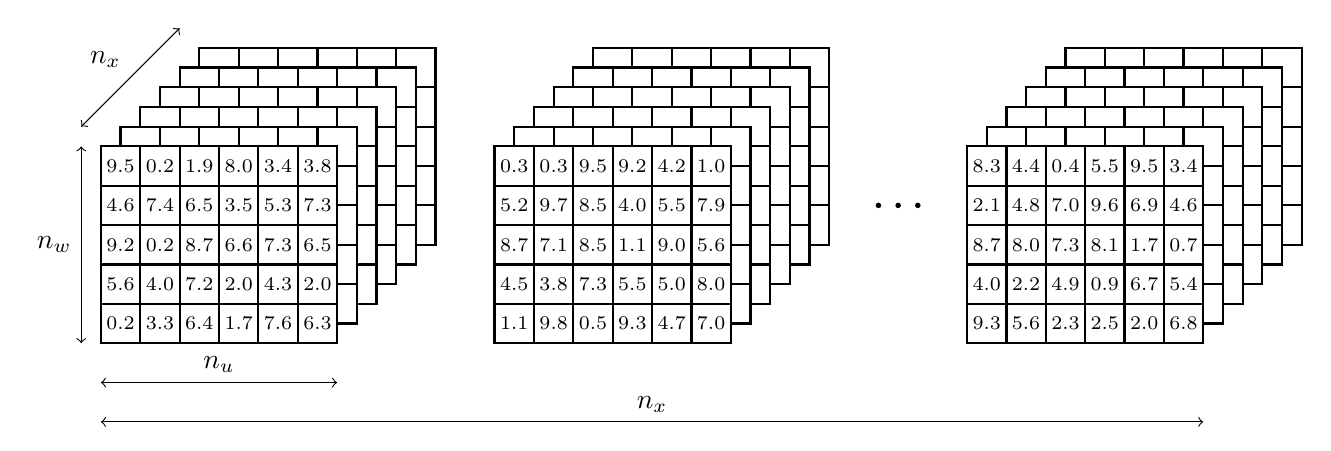
\begin{tikzpicture}

	\draw[thick,fill=white] (1.25,1.25) rectangle ++(3,2.5);
	\draw[step=0.5,thick,xshift=0.25cm,yshift=0.25cm] (1.0,1.0) grid ++(3,2.5);
	\draw[thick,fill=white] (1.0,1.0) rectangle ++(3,2.5);
	\draw[step=0.5,thick] (1.0,1.0) grid ++(3,2.5);	
	\draw[thick,fill=white] (0.75,0.75) rectangle ++(3,2.5);
	\draw[step=0.5,thick,xshift=0.25cm,yshift=0.25cm] (0.5,0.5) grid ++(3,2.5);
	\draw[thick,fill=white] (0.5,0.5) rectangle ++(3,2.5);
	\draw[step=0.5,thick] (0.5,0.5) grid ++(3,2.5);	
	\draw[thick,fill=white] (0.25,0.25) rectangle ++(3,2.5);
	\draw[step=0.5,thick,xshift=0.25cm,yshift=0.25cm] (0.0,0.0) grid ++(3,2.5);
	\draw[thick,fill=white] (0.0,0.0) rectangle ++(3,2.5);
	\draw[step=0.5,thick] (0.0,0.0) grid ++(3,2.5);	
	
	\node at (0.25,0.25) {\scriptsize 0.2};
	\node at (0.75,0.25) {\scriptsize 3.3};
	\node at (1.25,0.25) {\scriptsize 6.4};
	\node at (1.75,0.25) {\scriptsize 1.7};	
	\node at (2.25,0.25) {\scriptsize 7.6};
	\node at (2.75,0.25) {\scriptsize 6.3};
	
	\node at (0.25,0.75) {\scriptsize 5.6};
	\node at (0.75,0.75) {\scriptsize 4.0};
	\node at (1.25,0.75) {\scriptsize 7.2};
	\node at (1.75,0.75) {\scriptsize 2.0};	
	\node at (2.25,0.75) {\scriptsize 4.3};
	\node at (2.75,0.75) {\scriptsize 2.0};
	
	\node at (0.25,1.25) {\scriptsize 9.2};
	\node at (0.75,1.25) {\scriptsize 0.2};
	\node at (1.25,1.25) {\scriptsize 8.7};
	\node at (1.75,1.25) {\scriptsize 6.6};	
	\node at (2.25,1.25) {\scriptsize 7.3};
	\node at (2.75,1.25) {\scriptsize 6.5};
	
	\node at (0.25,1.75) {\scriptsize 4.6};
	\node at (0.75,1.75) {\scriptsize 7.4};
	\node at (1.25,1.75) {\scriptsize 6.5};
	\node at (1.75,1.75) {\scriptsize 3.5};	
	\node at (2.25,1.75) {\scriptsize 5.3};
	\node at (2.75,1.75) {\scriptsize 7.3};	
	
	\node at (0.25,2.25) {\scriptsize 9.5};
	\node at (0.75,2.25) {\scriptsize 0.2};
	\node at (1.25,2.25) {\scriptsize 1.9};
	\node at (1.75,2.25) {\scriptsize 8.0};	
	\node at (2.25,2.25) {\scriptsize 3.4};
	\node at (2.75,2.25) {\scriptsize 3.8};	
	
	\draw[thick,fill=white] (6.25,1.25) rectangle ++(3,2.5);
	\draw[step=0.5,thick,xshift=0.25cm,yshift=0.25cm] (6.0,1.0) grid ++(3,2.5);
	\draw[thick,fill=white] (6.0,1.0) rectangle ++(3,2.5);
	\draw[step=0.5,thick] (6.0,1.0) grid ++(3,2.5);	
	\draw[thick,fill=white] (5.75,0.75) rectangle ++(3,2.5);
	\draw[step=0.5,thick,xshift=0.25cm,yshift=0.25cm] (5.5,0.5) grid ++(3,2.5);
	\draw[thick,fill=white] (5.5,0.5) rectangle ++(3,2.5);
	\draw[step=0.5,thick] (5.5,0.5) grid ++(3,2.5);	
	\draw[thick,fill=white] (5.25,0.25) rectangle ++(3,2.5);
	\draw[step=0.5,thick,xshift=0.25cm,yshift=0.25cm] (5.0,0.0) grid ++(3,2.5);
	\draw[thick,fill=white] (5.0,0.0) rectangle ++(3,2.5);
	\draw[step=0.5,thick] (5.0,0.0) grid ++(3,2.5);	
	
	\node at (5.25,0.25) {\scriptsize 1.1};
	\node at (5.75,0.25) {\scriptsize 9.8};
	\node at (6.25,0.25) {\scriptsize 0.5};
	\node at (6.75,0.25) {\scriptsize 9.3};	
	\node at (7.25,0.25) {\scriptsize 4.7};
	\node at (7.75,0.25) {\scriptsize 7.0};
	
	\node at (5.25,0.75) {\scriptsize 4.5};
	\node at (5.75,0.75) {\scriptsize 3.8};
	\node at (6.25,0.75) {\scriptsize 7.3};
	\node at (6.75,0.75) {\scriptsize 5.5};	
	\node at (7.25,0.75) {\scriptsize 5.0};
	\node at (7.75,0.75) {\scriptsize 8.0};
	
	\node at (5.25,1.25) {\scriptsize 8.7};
	\node at (5.75,1.25) {\scriptsize 7.1};
	\node at (6.25,1.25) {\scriptsize 8.5};
	\node at (6.75,1.25) {\scriptsize 1.1};	
	\node at (7.25,1.25) {\scriptsize 9.0};
	\node at (7.75,1.25) {\scriptsize 5.6};
	
	\node at (5.25,1.75) {\scriptsize 5.2};
	\node at (5.75,1.75) {\scriptsize 9.7};
	\node at (6.25,1.75) {\scriptsize 8.5};
	\node at (6.75,1.75) {\scriptsize 4.0};	
	\node at (7.25,1.75) {\scriptsize 5.5};
	\node at (7.75,1.75) {\scriptsize 7.9};	
	
	\node at (5.25,2.25) {\scriptsize 0.3};
	\node at (5.75,2.25) {\scriptsize 0.3};
	\node at (6.25,2.25) {\scriptsize 9.5};
	\node at (6.75,2.25) {\scriptsize 9.2};	
	\node at (7.25,2.25) {\scriptsize 4.2};
	\node at (7.75,2.25) {\scriptsize 1.0};	

	\fill[black] (9.875,1.75) circle (1pt);
	\fill[black] (10.125,1.75) circle (1pt);
	\fill[black] (10.375,1.75) circle (1pt);
	
	\draw[thick,fill=white] (12.25,1.25) rectangle ++(3,2.5);
	\draw[step=0.5,thick,xshift=0.25cm,yshift=0.25cm] (12.0,1.0) grid ++(3,2.5);
	\draw[thick,fill=white] (12.0,1.0) rectangle ++(3,2.5);
	\draw[step=0.5,thick] (12.0,1.0) grid ++(3,2.5);	
	\draw[thick,fill=white] (11.75,0.75) rectangle ++(3,2.5);
	\draw[step=0.5,thick,xshift=0.25cm,yshift=0.25cm] (11.5,0.5) grid ++(3,2.5);
	\draw[thick,fill=white] (11.5,0.5) rectangle ++(3,2.5);
	\draw[step=0.5,thick] (11.5,0.5) grid ++(3,2.5);	
	\draw[thick,fill=white] (11.25,0.25) rectangle ++(3,2.5);
	\draw[step=0.5,thick,xshift=0.25cm,yshift=0.25cm] (11.0,0.0) grid ++(3,2.5);
	\draw[thick,fill=white] (11.0,0.0) rectangle ++(3,2.5);
	\draw[step=0.5,thick] (11.0,0.0) grid ++(3,2.5);

	\node at (11.25,0.25) {\scriptsize 9.3};
	\node at (11.75,0.25) {\scriptsize 5.6};
	\node at (12.25,0.25) {\scriptsize 2.3};
	\node at (12.75,0.25) {\scriptsize 2.5};	
	\node at (13.25,0.25) {\scriptsize 2.0};
	\node at (13.75,0.25) {\scriptsize 6.8};
	
	\node at (11.25,0.75) {\scriptsize 4.0};
	\node at (11.75,0.75) {\scriptsize 2.2};
	\node at (12.25,0.75) {\scriptsize 4.9};
	\node at (12.75,0.75) {\scriptsize 0.9};	
	\node at (13.25,0.75) {\scriptsize 6.7};
	\node at (13.75,0.75) {\scriptsize 5.4};
	
	\node at (11.25,1.25) {\scriptsize 8.7};
	\node at (11.75,1.25) {\scriptsize 8.0};
	\node at (12.25,1.25) {\scriptsize 7.3};
	\node at (12.75,1.25) {\scriptsize 8.1};	
	\node at (13.25,1.25) {\scriptsize 1.7};
	\node at (13.75,1.25) {\scriptsize 0.7};
	
	\node at (11.25,1.75) {\scriptsize 2.1};
	\node at (11.75,1.75) {\scriptsize 4.8};
	\node at (12.25,1.75) {\scriptsize 7.0};
	\node at (12.75,1.75) {\scriptsize 9.6};	
	\node at (13.25,1.75) {\scriptsize 6.9};
	\node at (13.75,1.75) {\scriptsize 4.6};	
	
	\node at (11.25,2.25) {\scriptsize 8.3};
	\node at (11.75,2.25) {\scriptsize 4.4};
	\node at (12.25,2.25) {\scriptsize 0.4};
	\node at (12.75,2.25) {\scriptsize 5.5};	
	\node at (13.25,2.25) {\scriptsize 9.5};
	\node at (13.75,2.25) {\scriptsize 3.4};	

	\draw[<->] (-0.25,2.75) -- node[above left] {$n_x$} ++(1.25,1.25);
	\draw[<->] (0,-1) -- node[above] {$n_x$} ++(14,0);	
	\draw[<->] (0,-0.5) -- node[above] {$n_u$} ++(3,0);
	\draw[<->] (-0.25,0) -- node[left] {$n_w$} ++(0,2.5);

\end{tikzpicture}
\caption{A four-dimensional table.}
\label{tikz:4d_table}
\end{figure}

A 3D table can be considered as a stack of 2D tables. Likewise, a 4D table can be considered as a stack of 3D tables.\newpage

\section{Optimistic Policy Iteration}
\label{appendix_D}

\begin{algorithm}
	\caption{Optimistic Policy Iteration}
	\begin{algorithmic}[0] % 1 to show code line numbers
		\Function{Optimistic Policy Iteration}{}
		\State
		\State Initialize $V(s) = 0 \; \forall \; s \in \mathcal{S}$
		\State Load arbitrary initial policy $\pi_0$.
		\State Initialize $m$,\;$\epsilon_V$
		\While {true}			
		\State
		\Function{Policy Evaluation}{}
		\ForAll{$s \in \mathcal{S}$}
		\State $V_{\pi,new}(s) \mathrel{\reflectbox{\ensuremath{\mapsto}}} r+\gamma V_ {\pi,old}(s')$
		\EndFor
		\EndFunction
		\State
		\Function{Policy Improvement}{}
		\ForAll{$s \in \mathcal{S}$}
		\State sample $m$ actions $a_n(s)$
		\ForAll {$a_n$}
		\State $Q(s,a_n) = r + \gamma V(s')$
		\EndFor
		\State $a_{greedy}(s)=\underset{a_n}{\text{argmax}}[Q(s,a_n)]$
		\EndFor
		\EndFunction
			\State Train policy on $a_{greedy,new}$ to obtain $\pi_{new}$
		\State
		\If {$||a_{greedy,new}-a_{greedy,old}||_\infty = 0$}
		\State break
		\EndIf	
		\EndWhile
		\State
		\EndFunction
	\end{algorithmic}
	\label{algo:opi}
\end{algorithm}

\section{Scenario 1: Additional Results}

